%File: formatting-instruction.tex
\documentclass[letterpaper]{article}
\usepackage{aaai}
\usepackage{times}
\usepackage{helvet}
\usepackage{courier}
\usepackage{graphicx}
\usepackage{amsmath}
\usepackage{subcaption}
\usepackage{tikz}
\usepackage[square,numbers,sort&compress]{natbib}
\usetikzlibrary{positioning, shapes.geometric, arrows.meta}
\usepackage{hyperref}
\frenchspacing
\setlength{\pdfpagewidth}{8.5in}
\setlength{\pdfpageheight}{11in}
\pdfinfo{
/Title (Parameter-Efficient Fine-Tuning of RoBERTa using LoRA for Robust AGNews Classification)
/Author (Ali Hamza, Saad Zubairi)}
\setcounter{secnumdepth}{0}  

\begin{document}

\title{Parameter-Efficient Fine-Tuning of RoBERTa using LoRA for Robust AGNews Classification}

\author{Hamza, A., \& Zubairi, S. \\
Department of Electrical and Computer Engineering\\
New York University Tandon School of Engineering\\
\texttt{ah7072@nyu.edu | shz2020@nyu.edu}\\
\url{https://github.com/saadhzubairi/deep-learning-mini-projects/tree/Project-2}\\
}
\maketitle

\begin{abstract}
    \begin{quote}
    We systematically explore Low‑Rank Adaptation (LoRA) configurations, data augmentation, and regularization to fine‑tune RoBERTa‑base on AGNews under a 1 M–parameter budget. Our best model achieves 94.61 \% validation accuracy (loss 0.1704) with ~962 k trainable parameters but only a 0.8420 score on the hidden Kaggle test set, revealing a notable validation–generalization gap under strict constraints.
    \end{quote}
    \end{abstract}

\section{Introduction}
Text classification models deployed on resource-constrained devices or latency-sensitive applications demand efficiency in memory and computation. The standard AGNews corpus—comprising 120k training and 7.6k test samples across four categories (World, Sports, Business, Sci/Tech)—serves as a practical benchmark for evaluating models under such constraints.

While fully fine-tuning large pre-trained models like RoBERTa-base (125M parameters) can achieve high accuracy (often $>$94\%) on this dataset, the associated computational and storage costs are prohibitive for many applications, limiting iterative development and on-device adaptation.

Low-Rank Adaptation (LoRA)~\cite{hu2022lora} offers a compelling alternative by freezing the pre-trained weights and injecting small, trainable low-rank matrices into specific layers. This drastically reduces the number of trainable parameters needed for task adaptation. However, optimal configuration of LoRA (rank, target modules) combined with other training techniques (data handling, regularization) under a strict parameter budget (e.g., $<$1M) is often non-trivial and dataset-dependent.

\subsection{Architecture}
We adapt a pre-trained RoBERTa-base transformer (125M parameters) to the AGNews task using Low-Rank Adaptation (LoRA) within a 1M trainable parameter limit. LoRA introduces trainable low-rank matrices into selected weight matrices while freezing the original weights, updating parameters as:
\[
W' = W + \alpha AB
\]
where $A \in \mathbf{R}^{d \times r}$, $B \in \mathbf{R}^{r \times d}$, rank $r$ controls adaptation capacity, and scaling factor $\alpha$ modulates update magnitude without affecting parameter count.

\paragraph{LoRA Parameterization:}
Each adapter adds $2dr$ parameters per matrix. For RoBERTa-base ($d=768$), total parameter count depends on:
\begin{itemize}
    \item \textbf{Rank ($r$):} Increasing $r$ linearly scales parameters (one layer with all 6 modules adds $13,824\cdot r$ parameters).
    \item \textbf{Target Modules:} Attention projections (\texttt{q\_proj}, \texttt{k\_proj}, \texttt{v\_proj}, \texttt{out\_proj}) and optionally FFN layers (\texttt{intermediate.dense}, \texttt{output.dense}).
    \item \textbf{Classifier Head:} Adapting the classifier (\texttt{dense}, \texttt{out\_proj}) adds approximately $2,300\cdot r$ parameters, minimal compared to encoder layers.
    \item \textbf{Layers Adapted:} Applying LoRA to all 12 encoder layers multiplies cost accordingly.
\end{itemize}

This structured approach ensures efficient adaptation of RoBERTa-base within strict parameter constraints while retaining substantial representational capacity.

\section{Methodology}

We fine-tuned RoBERTa-base to achieve optimal validation accuracy and minimal validation loss within a strict 1M parameter limit, emphasizing generalization and robustness. We leveraged Low-Rank Adaptation (LoRA), complemented by various optimizers, schedulers, regularization, and data strategies, each selected based on established literature.

\subsection{LoRA Configuration} LoRA efficiently reduces trainable parameters by injecting low-rank updates into frozen pre-trained weights \cite{hu2022lora}. Configuring LoRA required careful tuning of rank ($r$), scaling factor ($\alpha$), and adapter placement.

\paragraph{Rank ($r$) and Scaling ($\alpha$):} Rank $r$ defines adapter capacity, directly influencing parameter count and expressivity \cite{hu2022lora}. Higher $r$ increases representational power but risks overfitting; lower $r$ supports parameter efficiency but may underfit. The scaling factor $\alpha$, proportional to $r$, stabilizes training dynamics by modulating update magnitude \cite{li2023lora}. We systematically explored ranks $r=2$ to $10$, adjusting $\alpha$ accordingly ranging from 12 to 32.

\paragraph{Adapter Placement:} LoRA adapters were strategically tested across critical modules to effectively utilize the limited parameter budget:

\begin{itemize}
    \item \textbf{Attention Layers:} Adapting \texttt{q\_proj}, \texttt{k\_proj}, \texttt{v\_proj}, and \texttt{out\_proj} affects the model’s token-to-token interaction capabilities, enhancing context-specific feature extraction and attention mechanisms essential for capturing semantic relationships between words~\cite{vaswani2017attention}.
    \item \textbf{Feed-Forward Layers:} Applying LoRA to the \texttt{intermediate.dense} and \texttt{output.dense} layers targets intra-token transformations, refining token-level feature representations that are crucial for modeling the internal structure and nuanced meanings within tokens~\cite{liu2019roberta}.
    \item \textbf{Classifier Head:} Adapters on \texttt{classifier.dense} and \texttt{classifier.out\_proj} directly modulate the decision boundaries and label distributions, providing a focused and efficient adjustment of the model's final prediction outputs, particularly beneficial for fine-tuning to specific downstream tasks~\cite{kovaleva2019revealing}.
\end{itemize}

Early-layer adaptation is theoretically crucial for effective domain adaptation, while classifier tuning directly influences decision boundaries \cite{howard2018universal}.

\subsection{Optimizers and Learning Rate Scheduling}
We selected AdamW as the primary optimizer due to its proven effectiveness in transformer-based model fine-tuning, combining adaptive gradient-based optimization with weight decay regularization to enhance convergence stability and generalization~\cite{loshchilov2017decoupled}. We evaluated alternative optimizers such as AdaGrad and RMSProp; however, neither demonstrated improvements over AdamW in terms of validation accuracy or training efficiency.

For learning rate scheduling, we employed a linear decay scheduler with an initial warmup phase, which has consistently shown improved convergence stability and performance in transformer models by gradually adjusting the learning rate to mitigate early-stage instability~\cite{liu2019roberta}. Experiments with cosine annealing schedulers did not provide consistent or significant performance benefits compared to the linear schedule, validating our default choice.

\subsection{Regularization Techniques}
To enhance generalization and reduce the risk of overfitting within our constrained training regime, we applied targeted regularization methods:
\begin{itemize}
    \item \textbf{Dropout:} Implemented consistently within LoRA adapters and the classifier head, dropout randomly sets neurons to zero during training, promoting model robustness by preventing over-reliance on specific features~\cite{srivastava2014dropout}.
    \item \textbf{Label Smoothing:} By smoothing target labels and distributing a small portion of the target probability across all classes, label smoothing discourages overly confident predictions, thus encouraging better-calibrated output probabilities and improved generalization to unseen data~\cite{szegedy2016rethinking}.
\end{itemize}

\subsection{Data Augmentation and Filtering}
To enhance robustness and generalization, we implemented dynamic textual augmentation methods inspired by successful strategies in both NLP and computer vision literature \cite{wei2019eda, cubuk2019autoaugment}. Specifically, we employed:
\begin{itemize}
    \item \textbf{Synonym Replacement:} Randomly replacing selected words with their synonyms from WordNet introduces semantic diversity, thereby reducing the model's sensitivity to specific lexical choices and improving semantic generalization \cite{zhang2015character}.

    \item \textbf{Word Dropout:} Randomly removing words simulates incomplete or noisy input, compelling the model to rely less on specific words and more on context, thus increasing its robustness to fragmented or partial text \cite{iyyer2015deep}.

    \item \textbf{Random Swap:} Swapping the positions of two random words within a sentence helps simulate casual or informal writing variations, training the model to better handle grammatical inconsistencies common in real-world text data \cite{wei2019eda}.

    \item \textbf{Character-level Noise Injection:} Introducing small perturbations (substitution, capitalization, deletion, swapping, and special character insertion) mimics typographical errors and casual user-generated text, significantly enhancing the model's resilience to minor textual corruptions \cite{belinkov2018synthetic}.
\end{itemize}

Additionally, to improve dataset quality and reduce noise without sacrificing significant diversity, basic filtering techniques were applied:
\begin{itemize}
    \item \textbf{Text Length Filtering:} Samples exceeding 100 words were discarded, as excessively long texts might introduce noise or irrelevant details.
    \item \textbf{Non-Alphanumeric Ratio Filtering:} Texts with excessive non-alphanumeric characters (often indicative of corrupted or malformed inputs) were removed to maintain dataset integrity and readability.
\end{itemize}
These combined augmentation and filtering strategies systematically aimed at enhancing robustness and generalization of our model under strict computational constraints.

\section{Iterative Model Improvements}

We conducted systematic experiments to optimize validation accuracy while maintaining fewer than 1 million trainable parameters. Each configuration provides insights into parameter-efficient fine-tuning of pretrained language models:

\textbf{Baseline Model:} We applied LoRA adapters to attention components (query and value) of RoBERTa-base. With rank $r=8$ and scaling factor $\alpha=16$, this configuration achieved 94.34\% validation accuracy and a Kaggle score of 0.8418, while training only 888,580 parameters (0.71\% of total model parameters).
\textbf{Parameter Scaling (Models 2-3):} We investigated the impact of increasing LoRA hyperparameters:
\begin{enumerate}
    \item \textbf{Model 2: } Increasing rank to $r=10$ while maintaining $\alpha=16$ yielded modest improvement to 94.37\% validation accuracy with 962,308 parameters (0.77\%).
    
    \item \textbf{Model 3 (Final Kaggle Submission):} Further increasing scaling factor to $\alpha=32$ produced our highest Kaggle score (0.8420) with 94.61\% validation accuracy, demonstrating effective generalization and robustness. This configuration maintained 962,308 parameters (0.77\%).
\end{enumerate}
These experiments revealed diminishing returns from parameter scaling alone, suggesting the need for structural innovations beyond simple capacity increases.
\begin{figure}[h]
    \centering
    \begin{subfigure}[b]{0.15\textwidth}
        \centering
        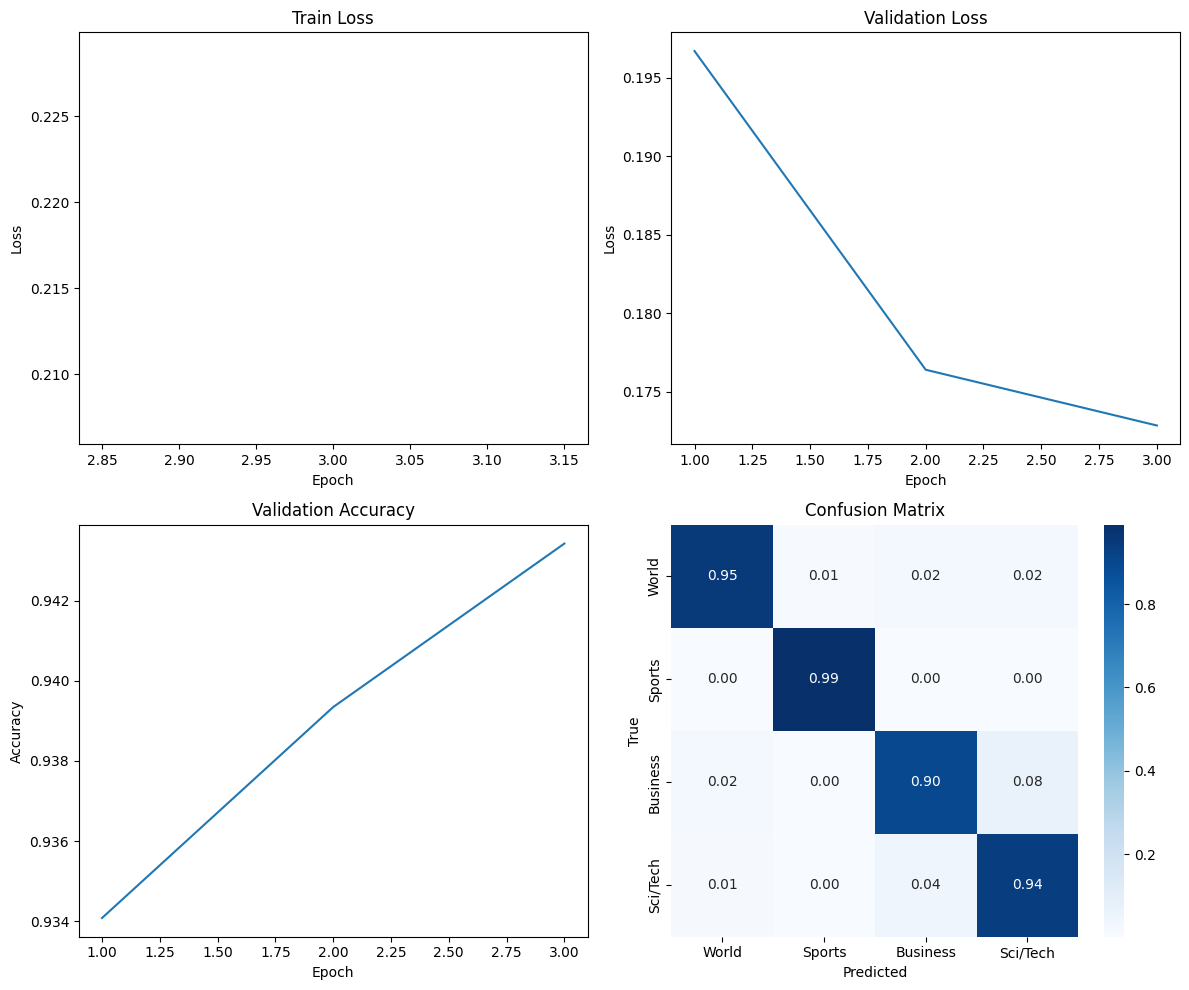
\includegraphics[width=\linewidth]{images/baseline.png}
        \caption{Baseline}
        \label{fig:baseline}
    \end{subfigure}
    \begin{subfigure}[b]{0.15\textwidth}
        \centering
        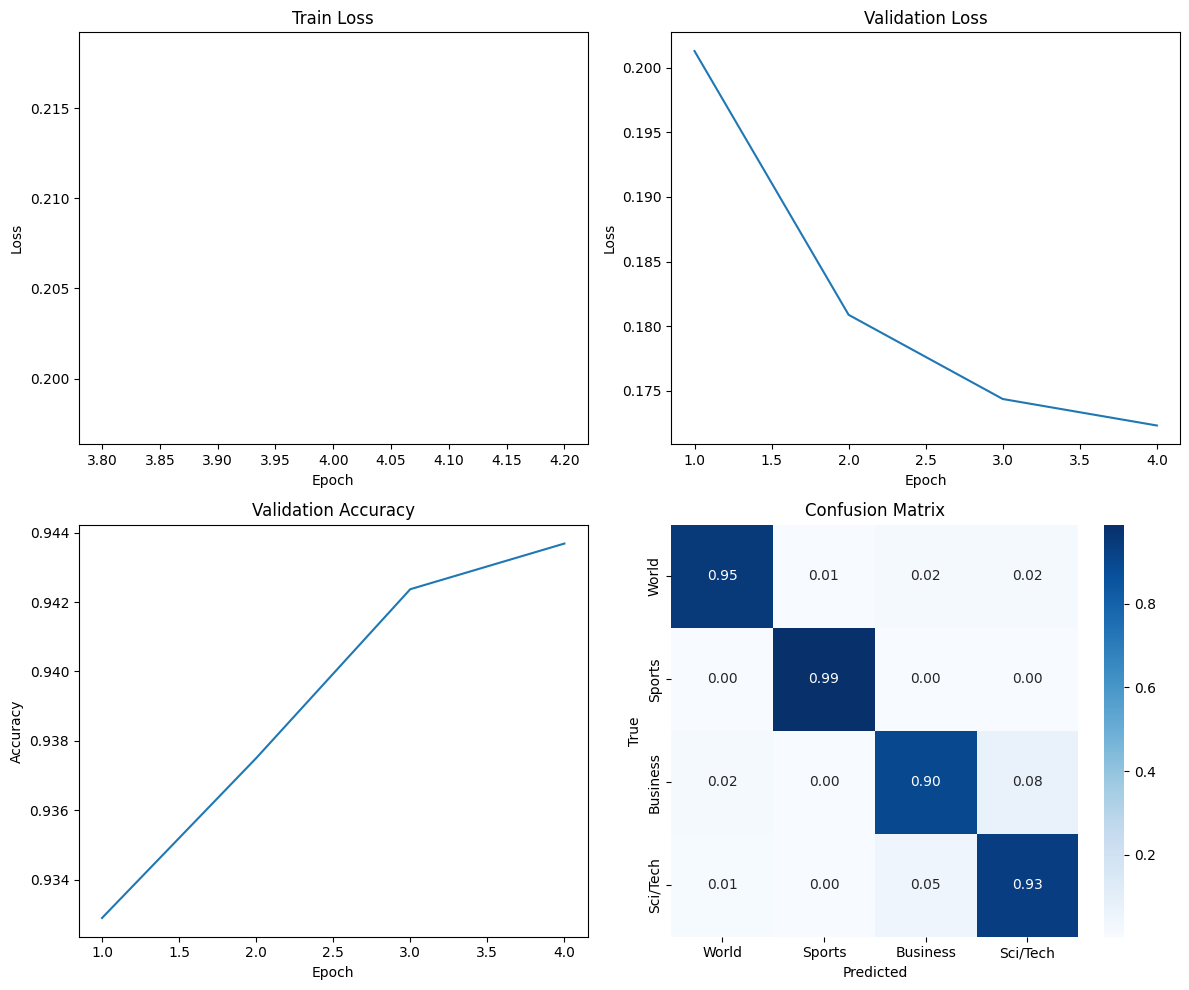
\includegraphics[width=\linewidth]{images/model_2.png}
        \caption{Model 2}
        \label{fig:model2}
    \end{subfigure}
    \hfill
    \begin{subfigure}[b]{0.15\textwidth}
        \centering
        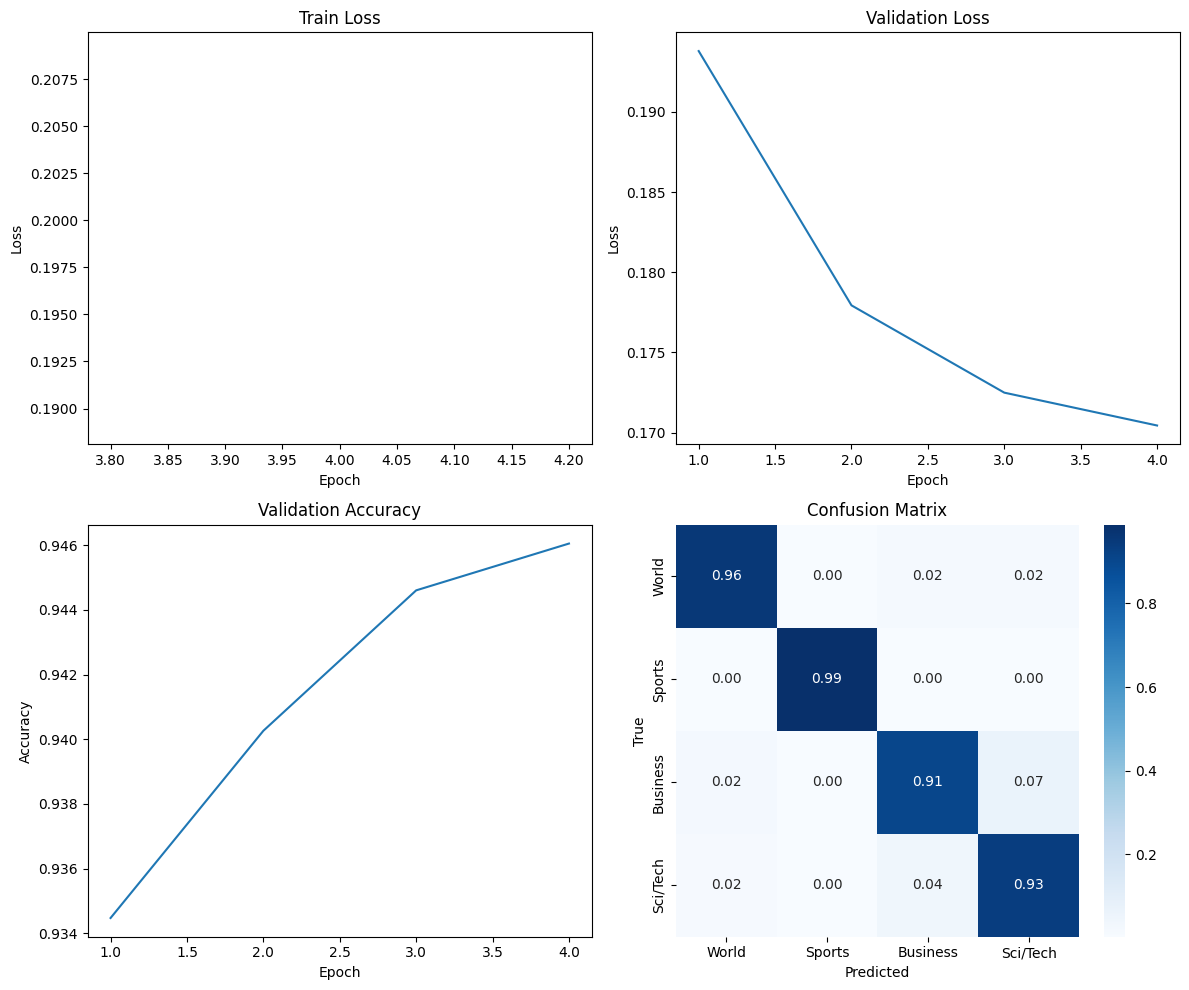
\includegraphics[width=\linewidth]{images/model_3.png}
        \caption{Model 3}
        \label{fig:model3}
    \end{subfigure}
    \caption{Comparison of learning curves for Models 2 and 3}
    \label{fig:rank-exp}
\end{figure}
\paragraph{Optimizer and Scheduler Variations (Models 4--6):} We evaluated alternative optimization approaches, including AdaGrad, RMSProp, and CosineAnnealingLR scheduling. These experiments yielded only marginal improvements (maximum validation accuracy of 94.58\%), confirming AdamW with linear scheduling as a robust default for LoRA fine-tuning so we did not pursue these further and did not include them in the final submission.
\paragraph{Module Expansion and Classifier Adaptation (Models 7--9):} We explored architectural variations in LoRA application:
\begin{enumerate}
    \item \textbf{Model 7:} Expanding adaptation to [query, key, value, intermediate.dense, output.dense] with conservative hyperparameters ($r=2$, $\alpha=12$) achieved 94.87\% validation accuracy with 925,444 parameters (0.74\%) however Kaggle performance dropped to 0.2670. 
    
    \item \textbf{Model 8:} Redirecting adaptation to [query, value, intermediate.dense, classifier.dense, classifier.out\_proj] with increased capacity ($r=4$, $\alpha=24$) yielded 94.63\% validation accuracy with 934,676 parameters (0.75\%) but a further drop in Kaggle performance to 0.2110. This configuration notably removed adaptation from the key attention component while adding adaptation to classifier-specific layers. 
    
    \item \textbf{Model 9:} Further concentrating adaptation on fewer modules [query, value, classifier.dense, classifier.out\_proj] with significantly higher capacity ($r=10$, $\alpha=32$) was tested to investigate the trade-off between module coverage and per-module adaptation depth but this produced worse validation accuracy (94.61\%) and was not submitted to Kaggle but the python notebook shows that this change deteriorated performance on the kaggle test set significantly.
\end{enumerate}

Despite impressive validation metrics, Models 7 and 8 exhibited substantial degradation in Kaggle performance (0.2110--0.2670), revealing a critical disconnect between validation and generalization performance. This decline was particularly pronounced when adaptation was applied to classifier components, supporting the hypothesis that classifier-focused adaptation promotes overfitting by enhancing task-specific features rather than improving general-purpose representations \citep{hu2022lora}.

\begin{figure}[h]
    \centering
    \begin{subfigure}[b]{0.15\textwidth}
        \centering
        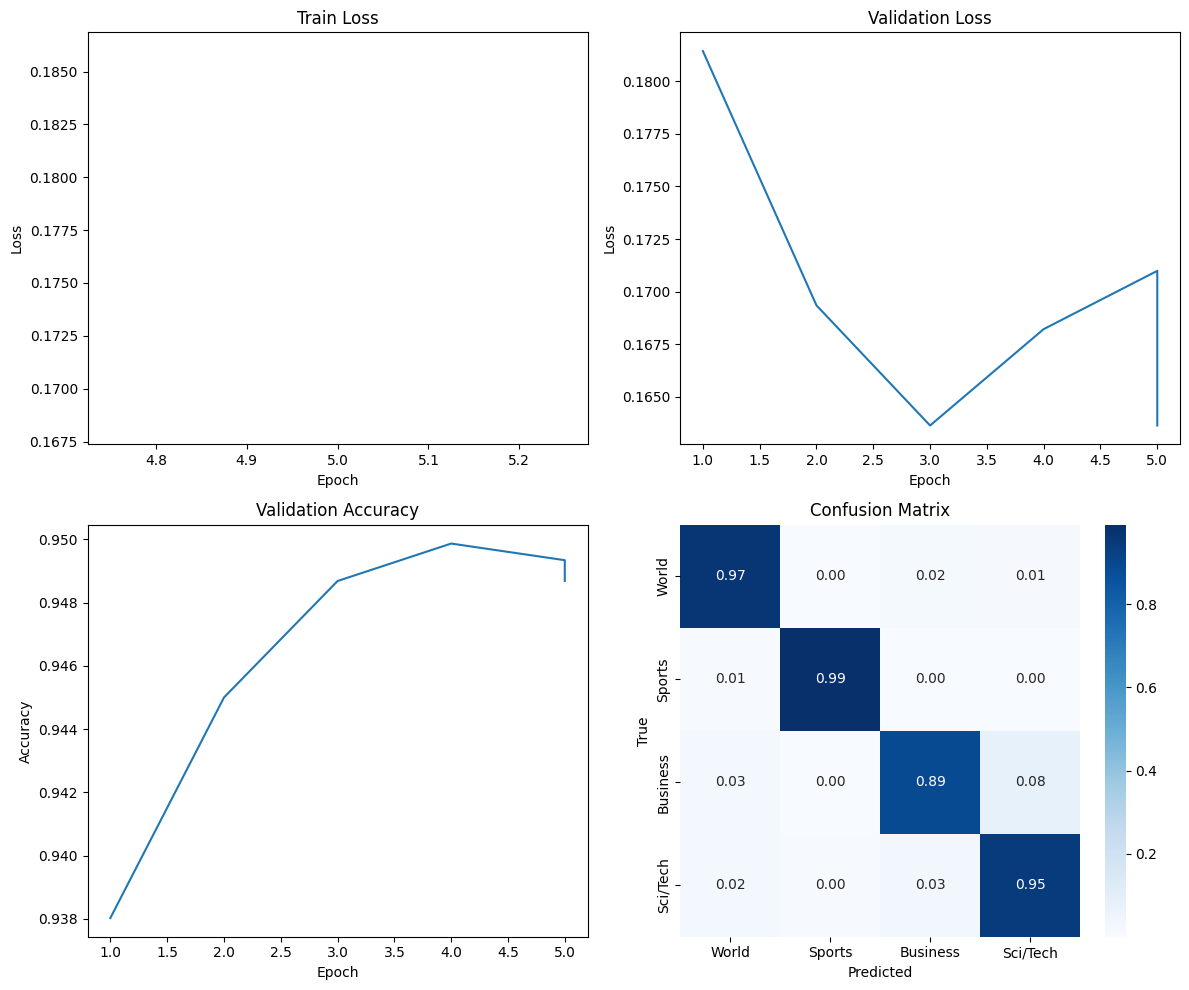
\includegraphics[width=\linewidth]{images/model_4.png}
        \caption{Model 7: Attention and FFN adaptation.}
        \label{fig:model7}
    \end{subfigure}
    \hfill
    \begin{subfigure}[b]{0.15\textwidth}
        \centering
        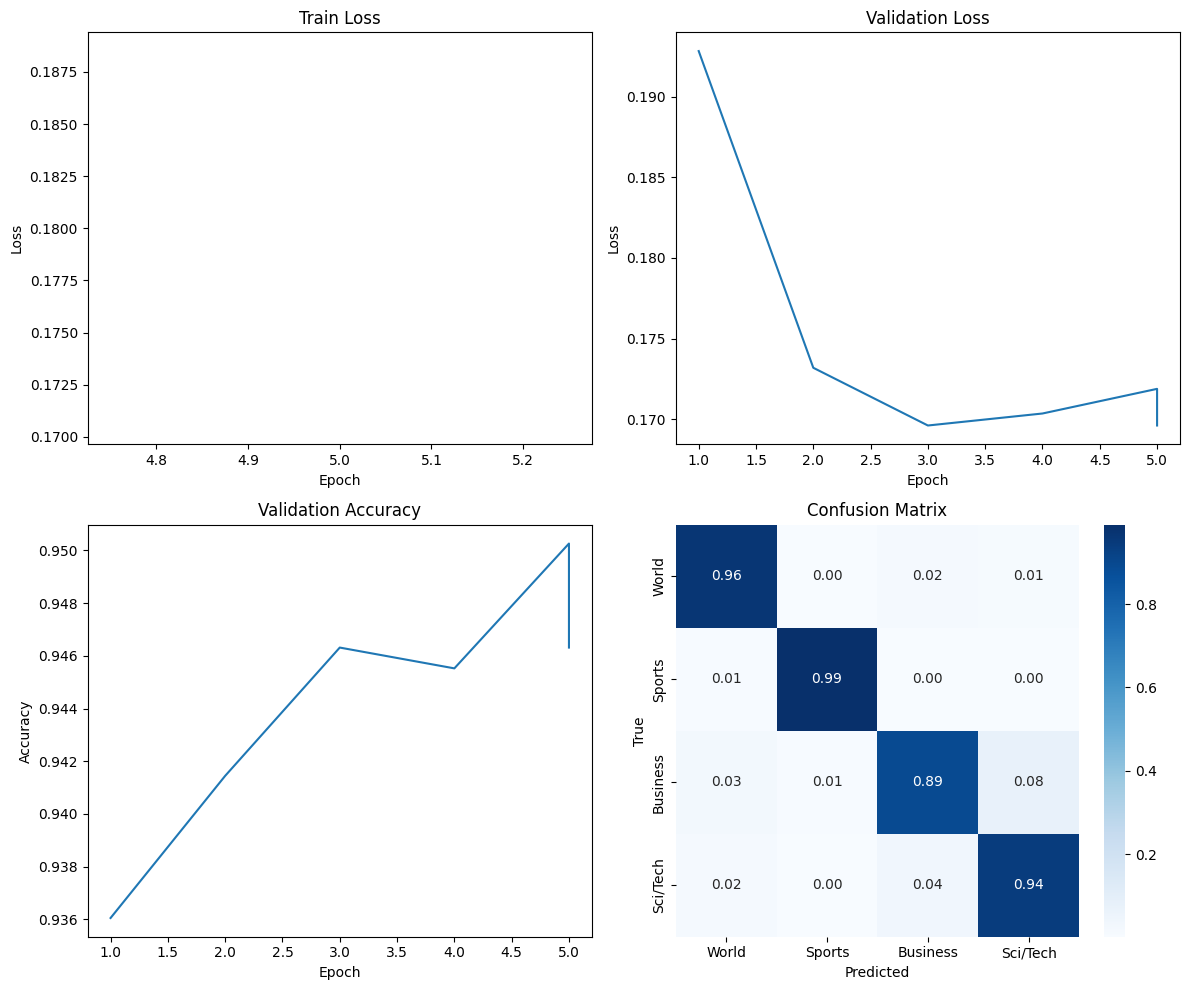
\includegraphics[width=\linewidth]{images/model_5.png}
        \caption{Model 8: Attention, FFN, and Classifier adaptation.}
        \label{fig:model8}
    \end{subfigure}
    \begin{subfigure}[b]{0.15\textwidth}
        \centering
        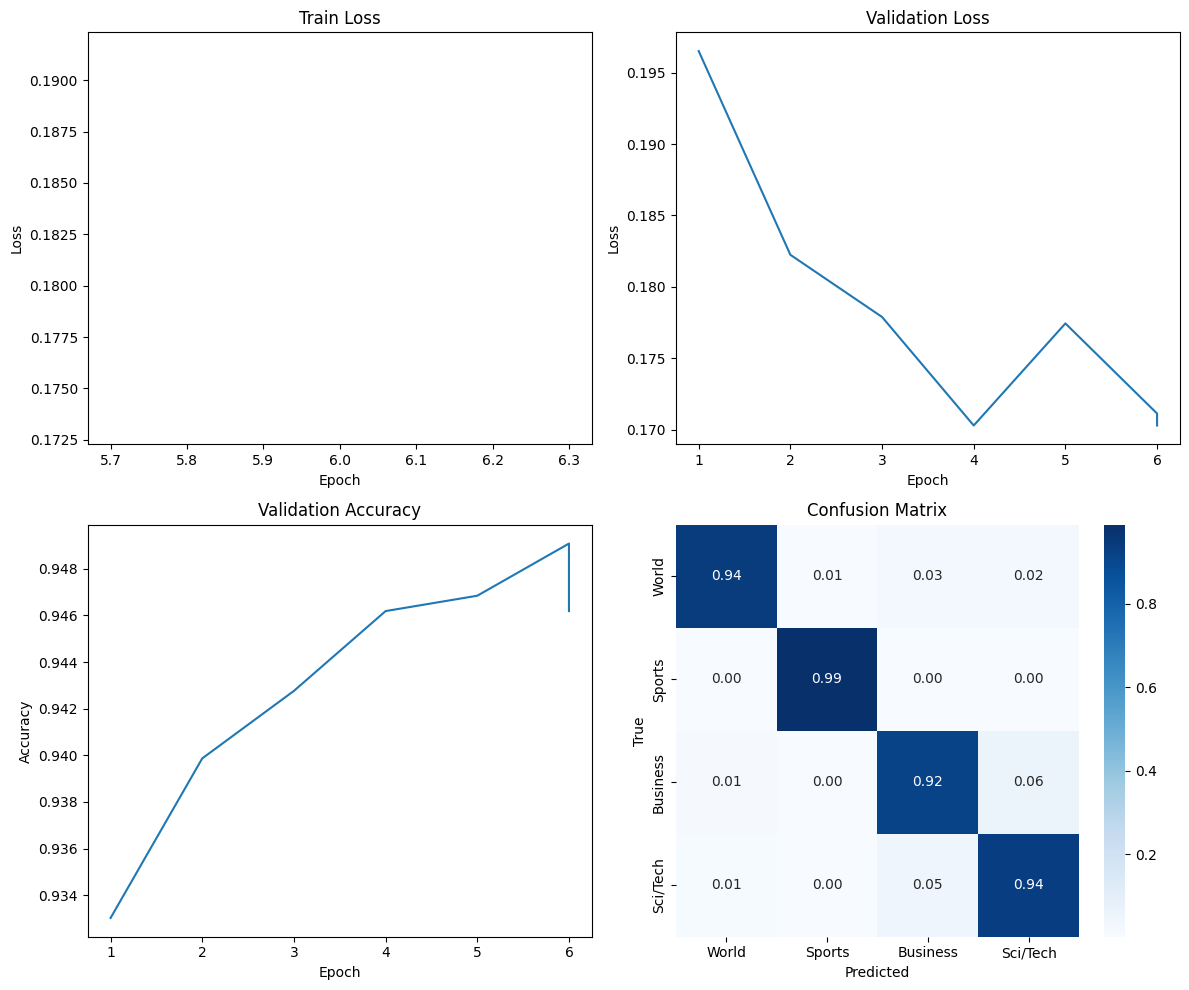
\includegraphics[width=\linewidth]{images/model_6.png}
        \caption{Model 9: Attention, and Classifier adaptation.}
        \label{fig:model9}
    \end{subfigure}
    \caption{Comparison of learning curves for Models 7, 8, and 9. The performance drop in Kaggle scores highlights the risk of overfitting when adapting classifier components.}
    \label{fig:module-adaptation}
\end{figure}

\paragraph{Data Augmentation and Regularization (Models 10--11):} We investigated complementary approaches to reduce overfitting in order to be able to adapt the classifier without overfitting:
\begin{enumerate}
    \item \textbf{Model 10:} We employed comprehensive text augmentation (synonym replacement, random swapping, dropout noise, character-level perturbations) with conservative filtering ($\leq$ 100 words, $\leq$ 10\% non-alphabetic characters) while maintaining the architecture from Model 9 to isolate data augmentation effects. This configuration achieved 94.56\% validation accuracy with 985,000 parameters (0.79\%) but did not yield an improvement to the models classification performance on the Kaggle test set.
    
    \item \textbf{Model 11:} We explored a contrasting approach by removing all data constraints while enhancing model-level regularization (dropout 0.15, warmup ratio 0.15, label smoothing 0.1) to compare model-based versus data-based interventions however based on the previous regularization approach we did not expect this to yield significant improvements. This configuration produced a model with 985,000 parameters (0.79\%) which was not tested
\end{enumerate}

These experiments contrast two complementary approaches to improving generalization: curating cleaner training signals through explicit data preprocessing versus relying on model-level regularization to extract robust features from noisy data. These experiments aimed to mitigate overfitting in a higher capacity model with classifier adaptation but the results were not positive.

\section{Discussion}
Our systematic exploration of parameter-efficient fine-tuning for RoBERTa-base on AGNews reveals several important insights:
\begin{table}[htbp]
    \centering
    \small
    \begin{tabular}{l|c|c|c|c}
         \textbf{Config} & \textbf{Params} & \textbf{Val Acc.} & \textbf{Val Loss} & \textbf{Kaggle} \\
         \hline
         Baseline & 888k & 0.943421 & 0.172851 & 0.8418 \\
         \hline
         $r$=10, $\alpha$=16 & 962k & 0.943684 & 0.172327 & - \\
         $r$=10, $\alpha$=32 & 962k & 0.946053 & 0.170443 & 0.8420 \\
         \hline
         attn+ffn& 925k & 0.948684 & 0.163645 & 0.2670 \\
         attn+ffn+cls& 934k & 0.946316 & 0.169608 & 0.2110 \\
         attn+cls& 985k & 0.946184 & 0.170281 & - \\
         \hline
         data aug+cls & 985k & 0.945658 & 0.169912 & - \\
         reg+cls & 985k & - & - & - \\
    \end{tabular}
    \caption{Model configuration comparison showing parameter count, validation metrics, and Kaggle scores. The most significant performance drop occurred when adaptation focused on classifier components (Models 7-8), despite strong validation metrics.}
    \label{tab:model_comparison}
\end{table}

\textbf{Parameter Efficiency vs. Generalization}
The most significant finding is the striking disparity between validation and test performance with certain adaptation strategies. While Models 7 and 8 achieved validation accuracy exceeding 94.8\%, their Kaggle performance deteriorated dramatically (0.2670 and 0.2110) compared to our baseline. This suggests validation metrics alone can be misleading indicators of generalization capability in parameter-constrained settings.

This performance gap was most pronounced when adaptation targeted task-specific components like classifier layers. This aligns with \cite{hu2022lora}, that adapting classifier components might capture dataset-specific patterns rather than generalizable representations.

\textbf{Strategic Module Selection}

Our experiments demonstrate that which modules to adapt matters more than parameter count or adapter rank. Adapting attention components yielded robust generalization across datasets, while redirecting adaptation to classifier components deteriorated generalization despite strong validation metrics.

The attention mechanism's ability to dynamically adjust context aggregation appears fundamental to robust adaptation, while task-specific layers seem more prone to dataset-specific overfitting.

\section{Conclusion}

This work investigated parameter-efficient fine-tuning of RoBERTa-base for AGNews classification using LoRA under a strict 1M parameter constraint. Our key conclusions:

\begin{itemize}
    \item Effective parameter-efficient adaptation depends more on strategic module selection than raw parameter count, with attention components proving consistently superior for generalization.
    
    \item A significant validation-generalization gap emerges with certain adaptation strategies, revealing limitations in standard evaluation practices.
    
    \item Parameter scaling alone yields diminishing returns beyond certain thresholds, which in our case was 10, suggesting fundamental limitations to capacity-focused approaches.
\end{itemize}

\textbf{Limitations and Future Work}

This study was limited to a single dataset and model architecture. Future work should expand to diverse tasks and models, conduct controlled experiments with artificial distribution shifts to better isolate factors affecting generalization, explore more sophisticated augmentation and regularization strategies, and compare LoRA with alternative parameter-efficient methods.

Despite these limitations, our work provides practical guidance for practitioners working with parameter-efficient fine-tuning methods under resource constraints. 

Furthermore, due to limitations of compute not all experiments could be conducted multiple times to ensure accuracy and robustness of results. The results presented here are based on a single run of each configuration, and further validation is needed to confirm the findings.

\bibliography{references}
\bibliographystyle{abbrv}

\end{document}
